\section{Object Re-identification Datasets}
\label{sec:ObjectReIDDatasets}

% ##############################################################################
\subsection{VeRI-776}
\label{ssec:DatasetVeRI776}

A large-scale benchmark dataset named \verisss{} for vehicle \gls{reid} in the real-world urban surveillance scenario~\cite{liu2018provid} (\figtext{}~\ref{fig:VeRI776Dataset}). In our opinion, this dataset is one of the best available, and it already has been explored and served the purpose of training \gls{reid} models. The featured properties of this include the following important properties for training robust \gls{reid} models:

\begin{itemize}
    \item It contains over $50\ 000$ images of $776$ vehicles captured by $20$ cameras covering an $1\  \text{km}^2$ area in $24$ hours.
    \item The images were captured in a real-world unconstrained surveillance scene and labeled with varied attributes, \egtext{}, \glspl{bbox}, types, colors, and brands.
    \item Each vehicle is captured by at least $2$ up to $18$ cameras in different viewpoints, illuminations, resolutions, and occlusions.
    \item Data samples are also labeled with license plates and other spatio-temporal information, such as the \glspl{bbox} of plates with corresponding strings, the timestamps of vehicles, and the distances between neighboring cameras.
\end{itemize}

% ------------------------------------------------------------------------------
\begin{figure}[t]
    \centerline{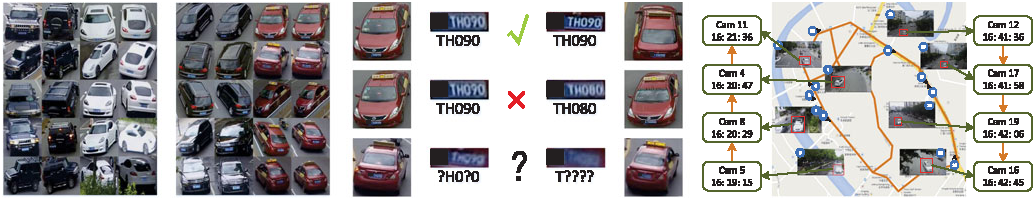
\includegraphics[width=\linewidth]{figures/datasets/veri776__overview.pdf}}
    \caption[\verisss{} dataset]{The properties of the \verisss{} dataset. Individual vehicles offer rich within-class differences in distinct viewpoints. At the same time, different but similar vehicles may have trivial inter-class differences. \externalsrc{\cite{liu2018provid}}}
    \label{fig:VeRI776Dataset}
\end{figure}
% ------------------------------------------------------------------------------
